\documentclass[12pt]{article}
\usepackage[margin=1.5cm]{geometry}
\usepackage{parskip}
\usepackage{amsmath}
\usepackage{amssymb}
\usepackage{amsfonts}
\usepackage{enumitem}
\usepackage{graphicx}
\usepackage{stmaryrd}
\graphicspath{ {./images/} }


\begin{document}
\begin{enumerate}[label=(\alph*)]
  \item
    In genome assembly, we can consider two different ways of generating graphs from reads of a DNA sequence to help us solve the genome assembly problem. We assume that we have a collection of $k$-mers from reads of a DNA sequence, which are $k$-letter sequences.

    The first way of doing this is treating $k$-mers as nodes. Each node in a graph can be a different $k$-mer, and we create an edge from $n_1$ to $n_2$ if $suffix(n_1) = prefix(n_2)$. At this point, we can reconstruct a genome by finding a path that visits every node, since this corresponds to all of the reads. This is the same as finding a Hamiltonian path in our graph.

    The second way of doing this is treating $k$-mers as edges. In this case, for a $k$-mer, we create two nodes, corresponding to the prefix and suffix of the $k$-mer, and draw an edge from the prefix node to the suffix node, where this edge is the $k$-mer. We can then compress this graph by joining together nodes with the same label. Then, reconstructing the genome then becomes equivalent to finding an Eulerian path in the graph.

  \item
    To apply De Bruijn graphs to genome assembly, we use the same technique as described in (a).

    First, we take our reads, and decompose them into $k$-mers. Then, we turn each $k$-mer into a prefix node, a suffix node, and an edge between them. We can then take all nodes with the same label and compress them together, forming a de Bruijn graph.

    At this point, reconstructing the genome is the same as finding an Eulerian path in the resulting de Bruijn graph.

    For example, suppose we start with genome \texttt{ATCATG}.
    
    This generates the following 2-mers:

\begin{verbatim}
AT
TC
CA
AT
TG
\end{verbatim}

This generates the following De Bruijn graph:

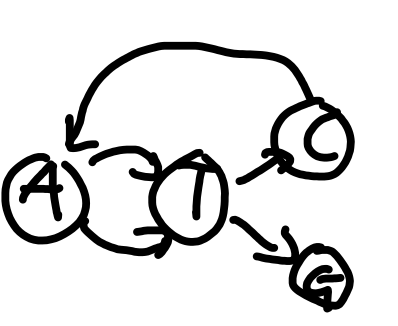
\includegraphics[scale=0.4]{debruijn}

We can then reconstruct the genome as an Eulerian path: \texttt{ATCATG}

\item
  By choosing a short $k$-mer length, we increase the number of possible Eulerian paths in our final De Bruijn graph (assuming we use that technique, although we get similar results for other techniques). This means that the accuracy of our genome reconstruction is lower since we are less likely to be able to reconstruct the actual original genome, and we may instead get some other variant.

  However, choosing a large $k$-mer length limits the amount of $k$-mers that we can obtain from a single read, so we may need to take more reads for a large $k$-mer length in order to be able to reconstruct the genome.

\item
  In phylogeny, a distance matrix is additive if there exists an unrooted tree that fits it, effectively meaning that the distances correspond to some actual measure of distance (to some extent). Algorithms like the additive phylogeny algorithm, and neighbour joining, are guaranteed to find such a tree if a distance matrix is additive, but if the distance matrix is not additive, then we may not be able to produce any tree (like in additive phylogeny) or settle for some tree that attempts to fit to the distance matrix as best as it can (like in neighbour joining).

\item
  The following is an additive distance matrix:

\begin{verbatim}
  A  B  C
A    5  10
B       15
C
\end{verbatim}

The following is not an additive distance matrix:

\begin{verbatim}
  A  B  C
A    5  10
B       1
C
\end{verbatim}


        
\end{enumerate}
\end{document}
